\documentclass[a4paper,twoside]{article}

\usepackage[a4paper, total={6in, 8in}]{geometry}

\usepackage{tkz-euclide}

\usepackage{amssymb}
\usepackage{amsfonts}
\usepackage{enumitem}
\usepackage{stmaryrd}
\usepackage{amsmath}
\usepackage{easybmat}
\usepackage{tikz}

%-------------------------------commands definitionen-------------------------------
% Für methoden die eine fallunterscheidung haben aufrufen mit: 
% \twopartdef 	{x} {x \geq 0} 
%				{-x} {x < 0} 
%(bsp. Betrag)
\newcommand{\twopartdef}[4] {
	\left\{
		\begin{array}{ll}
			#1 & #2 \\
			#3 & #4
		\end{array}
	\right.
}
% Für methoden mit 3 fällen zwischen denen entschieden werden muss
\newcommand{\threepartdef}[6] {
	\left\{
		\begin{array}{lll}
			#1 &  #2 \\
			#3 &  #4 \\
			#5 &  #6
		\end{array}
	\right.
}
% Am besten immer die befehle Einrücken, damit man erkennt welche Matrix dargestellt wird.
% Z.B.: \twoXtwo{1}{2}
%				{3}{4}
\newcommand{\twoXtwo}[4] {
	\left( 
	\begin{matrix}
		#1 & #2 \\
		#3 & #4
	\end{matrix} 
	\right)
}
\newcommand{\twoXthree}[6] {
	\left( 
	\begin{matrix}
		#1 & #2 & #3\\
		#4 & #5 & #6
	\end{matrix} 
	\right)
}
\newcommand{\threeXtwo}[6] {
	\left( 
	\begin{matrix}
		#1 & #2 \\
		#3 & #4 \\
		#5 & #6
	\end{matrix} 
	\right)
}
\newcommand{\threeXthree}[9] {
	\left( 
	\begin{matrix}
		#1 & #2 & #3\\
		#4 & #5 & #6\\
		#7 & #8 & #9\\
	\end{matrix}
	\right)
}
%Vektoren, sind quasi nx1 matrizen
\newcommand{\vecTwo}[2] {
	\left( 
	\begin{matrix}
		#1\\
		#2
	\end{matrix} 
	\right)
}
% Abkürzung von \textnormal
\newcommand{\tn}[1]{\textnormal {#1}}
%-----------------------------ende commands definitionen-----------------------------

\begin{document}

\title{Lineare Algebra II - Mitschrift}
\author{Sebastian Pretzsch, Finn Ribbeck, Jonas Heitz}
\maketitle
%------------------------------------Vorlesung 1------------------------------------
\section{Relationen}
Relationen beschreiben Beziehungen zwischen Elementen von Mengen. \\
Wdh. $X{\times}Y := \{(x,y) | x \in X, y \in Y\}$ \\
Menge der (geordneten) Paare, "kartesiches Produkt".

\subsection*{Definition 1.1.}
Seien X,Y Mengen. Eine \textbf{Relation} zwischen X und Y ist eine Teilmenge $R \subseteq X{\times}Y$. \\
\underline{Notation}: für $(x,y)\in R$ auch $xRy$. \\
Falls $X=Y$ sage auch Relation "auf X".

\subsection*{Beispiel}
$X$ Punktmenge, $Y$ Geradenmenge
$$xRy :\Leftrightarrow \tn{Punkt x liegt auf Gerade y}$$

\subsection*{Bemerkung}
Eine Abbildung (Funktion) $f:X{\to}Y$ weist zu jedem $x\in X$ genau ein $
y\in Y$ zu. \\
Wir werden diese fortan als spezielle Relation
$$R_f = \{(x, f(x)) | x\in X\} \subseteq X{\times}Y$$
auffassen. Wir betrachten insbesondere Relation auf X.

\subsection*{Definition 1.2.}
Sei X eine Menge. Eine Relation $R \subseteq X{\times}X$ ist
\begin{enumerate}[label=(\alph*)]
\item \textbf{reflexiv} falls $xRx \hspace*{2mm}\forall x\in X$,
\item \textbf{symmetrisch} falls $xRy \Rightarrow yRx \hspace*{2mm}\forall x,y\in X$ (denn auch "$\Leftarrow$" gilt),
\item \textbf{anti-symmetrisch} falls $xRy \land yRx \Rightarrow x=y$,
\item \textbf{transitiv} falls $xRy \land yRz \Rightarrow xRz$.
\end{enumerate}

\subsection*{Beispiel} 
Sei $X = \mathbb R$.
\begin{enumerate}[label=(\alph*)]
\item $ R:=\{(x,x) | x\in X\}$ (d.h. $xRy \Rightarrow x=y$) erfüllt a), b), c), d).
\item $ xRy :\Leftrightarrow |x|=|y|$ erfüllt a), b), d) (nicht c), da $|1|=|-1|$)
\item $ xRy :\Leftrightarrow x\leq y$ erfüllt a), c), d) (nicht b), da $2\leq 3$ aber $2 \neq 3$
\end{enumerate}
Nun definieren wir die wichtigsten Arten von Relationen.

\subsection*{Definition 1.3.}
Eine Relation R auf X heißt
\begin{enumerate}[label=(\arabic*)]
\item \textbf{Äquivalenzrelation} falls sie reflexiv, symmetrisch und transitiv ist (typische Notation "$\sim$"),
\item \textbf{Ordnungsrelation} falls sie reflexiv, anti-symmetrisch und transitiv ist (Notation "$\leq$").
\end{enumerate}
Im Fall 2. heißt R auch \textbf{(partielle) Ordnung}, und falls 
$$ xRy \lor yRx \hspace*{2mm} \forall x,y \in X$$
zusätzlich gilt \textbf{totale/ lineare Ordnung}.\\
\textbf{Äquivalenzrelationen} auf X entsprechen genau den Zerlegungen von X.
Zwei Mengen A, B heißen \textbf{disjunkt} falls $A \cap B = \emptyset$.

\subsection*{Beispiel}
Kleiner Ausblick:
\begin{enumerate}[label=(\alph*)]
\item Zwei Matrizen $A,B \in \tn{Mat}_{n{\times}m}(K)$ heißen \textbf{ähnlich} falls $S \in \tn{GL}_n(K)$ existiert mit \\$B=S^{-1}{\cdot}A{\cdot}S$.
\item Sei M Menge und $X:=\mathcal P(M)$ Potenzmenge von M\\
 Zu $A,B \in X$ definiere $A\leq B :\Leftrightarrow A\subseteq B$ eine Ordnungsrelation.
\end{enumerate}

%------------------------------------Vorlesung 2------------------------------------
\subsection*{Definition 1.4.}
Sei X Menge. Eine \textbf{Zerlegung} von X ist eine Menge $\mathcal{C}$ von paarweise disjunkten nicht-leeren Mengen $A \subseteq X$ mit $\bigcup_{A \in \mathcal{C}} A = X$.

\subsection*{Beispiel}
Eine Zerlegung von $\{ a, b, c\}$ ist $\{\{ a\}, \{ b, c\}\}$.

\subsection*{Lemma 1.5.}
Sei $\sim$ Äquivalenzrelation auf X und zu $x \in X$ sei $[x] := \{y \in X | x \sim y\} \subseteq X$ ("Klasse" von X).\newline
Dann ist $\mathcal{C} := \{[x] | x \in X\}$ eine Zerlegung von X.\newline
Ferner gilt $x \sim y \Leftrightarrow [x] =  [y]$. (*)\newline
\subsubsection*{Beweis (*)}
"$\Leftarrow$": $y \in [y] = [x] \Rightarrow x \sim y$.\newline
"$\Rightarrow$": Gelte $x \sim y$. Zeige [x] = [y].
\begin{itemize}
\item[--] "$\subseteq$": $z \in [x] \Rightarrow x \sim z \Rightarrow y \sim z \Rightarrow z \in [y]$
\item[--] "$\supseteq$": $z \in [y] \Rightarrow y \sim z \Rightarrow x \sim z \Rightarrow z \in [x]$\newline
\end{itemize}
Zeige $\mathcal{C}$ Zerlegung.\newline
Angenommen $[x] \cap [y] \neq \emptyset \Rightarrow \exists z \in X: z \in [x] \cap [y] \Rightarrow \exists z \in X: x \sim z \sim y \Rightarrow x \sim y \Rightarrow [x] = [y].$\newline Also sind die Klassen paarweise disjunkt (und nicht-leer, da $\forall x \in X: x \in [x]$).\newline Wegen $\forall x \in X: x \in [x]$ gilt außerdem $\bigcup_{x \in X} [x] = X$.

\begin{flushleft}
$\square$\\
\end{flushleft}

\subsection*{Beispiel}
\begin{enumerate}[label=(\alph*)]
\item $X = \mathbb{R}, x \sim y :\Leftrightarrow |x| = |y|$.
Zerlegung von $\mathbb{R}$ ist $\{\{0\}\} \cup \{\{a, -a\} | a \in \mathbb{R}_{>0}\}$.
\item $X = \mathbb{Z}, n \in \mathbb{N}_{>0}$, betrachte $x \sim y :\Leftrightarrow n | x - y \Leftrightarrow y = x + k \cdot n$ für ein $k \in \mathbb{Z}$.
Zerlegung von $\mathbb{Z}$ ist $\{0 + n\mathbb{Z},\ldots, (n - 1) + n\mathbb{Z}\}$ (n Klassen).
\end{enumerate}

\subsection*{Definition 1.6.}
Die Zerlegung von X bezüglich der Relation $\sim$ heißt Zerlegung in \textbf{Äquivalenzklassen}. Notation für $\mathcal{C}$ auch X/$\sim$, "X modulo $\sim$".
\subsubsection*{Bemerkung}
Umgekehrt definiert jede Zerlegung $\mathcal{C}$ von X Äquivalenzrelation $\sim_\mathcal{C} := \bigcup_{A \in \mathcal{C}} A \times A \subseteq X \times X$ (Übung) und die Konstruktionen sind zueinander invers.

\subsection*{Beispiel}
Es gibt fünf Zerlegungen von $X = \{a, b, c\}$. Die Kreuztabellen der zugehörigen Äquivalenzrelationen lauten:
\begin{tabbing}
\=
\begin{tabular}[h]{cccc}
 & a & b & c \\
a & X & & \\
b & & X & \\
c & & & X \\
\end{tabular}
\=
\begin{tabular}[h]{cccc}
 & a & b & c \\
a & X & X & \\
b & X & X & \\
c & & & X \\
\end{tabular}
\=
\begin{tabular}[h]{cccc}
 & a & b & c \\
a & X & & X \\
b & & X & \\
c & X & & X \\
\end{tabular}
\=
\begin{tabular}[h]{cccc}
 & a & b & c \\
a & X & & \\
b & & X & X \\
c & & X & X \\
\end{tabular}
\=
\begin{tabular}[h]{cccc}
 & a & b & c \\
a & X & X & X \\
b & X & X & X \\
c & X & X & X \\
\end{tabular}
\\
\>$\{\{a\}, \{b\}, \{c\}\}$
\>$\{\{a, b\}, \{c\}\}$
\>$\{\{a, c\}, \{b\}\}$
\>$\{\{b, c\}, \{a\}\}$
\>$\{\{a, b, c\}\}$\\
\end{tabbing}
Zusammenhang mit Abbildungen:
\subsubsection*{Bemerkung}
Jede Äquivalenzrelation $\sim$ auf X definiert eine (surjektive) Abbildung\\
$\pi: X \longrightarrow X/\sim, x \longmapsto [x]$.\\
Umgekehrt definiert jede Abbildung $f: X \longrightarrow Y$ eine Äquivalenzrelation auf X durch\\ $x \sim x' :\Leftrightarrow f(x) = f(x')$.

\subsection*{Wichtige Begriffe zu Ordnung}
Sei (X, $\leq$) geordnete Menge. Darstellung (im endlichen Fall) als Diagramm mit Verbindungen \begin{tabular}{c}
b \cr $\mid$ \cr a
\end{tabular} falls $a < b$ und es existiert kein $c$ mit $a < c < b$ "Nachbarschaftsrelation".

\subsection*{Beispiel}
siehe Vorlesung (15.04.21 / 56:20)

\subsection*{Definition 1.7.}
Sei (X, $\leq$) geordnete Menge. Elemente $a, b \in X$ heißen \textbf{vergleichbar} falls $a \leq b \lor b \leq a$.\\
Teilmenge $Y \subseteq X$ heißt \textbf{Kette} falls alle $a, b \in Y$ vergleichbar (d.h. X ist Kette gdw. X total geordnet).
\begin{tabbing}
Ein Element $a \in X$ heißt \= \textbf{maximal} falls $\forall x \in X: x \geq a \Rightarrow x = a$,\\ \>\textbf{größtes Element} falls $\forall x \in X: x \leq a$.\\ \>\textbf{obere Schranke} von $Y \subseteq X$ falls $\forall y \in Y: y \leq a$.\\
Dual dazu: minimal, kleinstes Element, untere Schranke\\
\end{tabbing}

\subsection*{Beispiel}
$\mathcal{P}(M)\backslash\{\emptyset\}$ hat als minimale Elemente $\{m\}$ wobei $m \in M$.\\
z.B.: $M:=\{a, b\} \rightarrow \mathcal{P}(M)\backslash\{\emptyset\} = \{\{a\}, \{b\}, \{a, b\}\}$ hat minimale Elemente $\{a\}$ und $\{b\}$.
%----------------------------------Vorlesung 3----------------------------------
\section{Unendliche Mengen und Lemma von Zorn}
Notation: Zu $n\in\mathbb{N}$ sei $[n]:= \{1,2...,n\} $.

\subsection*{Definition 2.1.}
Eine Menge $X$ heißt endlich, falls $\exists n \in \mathbb{N}$ und Bijektion $\phi: X \rightarrow [n]$; in diesem Fall heißt $n$ die Kardinalität $|X|$ oder $\#X$ von $X$.
Ansonsten heißt $X$ unendlich. 
\subsubsection*{Bemerkung (Taubenschlagprinzip)}
Ist $n>m$, so ist jede Abbildung $f: [n] \rightarrow [m]$ nicht injektiv, das heißt $\exists x\neq x'$ ("Tauben") mit $f(x) = f(x')$. \\
Es folgt: Ist $\phi : [n] \rightarrow [m]$ bijektiv, so gilt $n=m$. Somit ist die Kardinalität eindeutig.

\subsection*{Beispiel}
Menge $X = \{a,b,c,d\}$ ist endlich mit Kardinalität 4, \\
$\#X =  4$ mögliche Bijektion: 
\begin{tabular}{cccc}
$a \rightarrow 1$ & $c \rightarrow 3$ \\
$b \rightarrow 2$ & $d \rightarrow 4$ \\
\end{tabular}
\\
\\
Der Umgang mit unendlichen Mengen erfordert oft "Auswahlaxiom".

\subsection*{Bemerkung}
Abbildung $f: X \rightarrow Y$ ist injektiv $\Leftrightarrow \exists g: Y \rightarrow X : g \circ f = id_x$ ($X \neq \emptyset $).
\subsubsection*{Beweis}
$"\Leftarrow"$ \\
$x,x' \in X :$
$f(x) = f(x') \Rightarrow  x = g(f(x)) = g(f(x'))$ nach Voraussetzung.\\
Also ist f injektiv. \\ 
\\
$"\Rightarrow"$\\
Sei $Y_0 := im f$ und betrachte $f_0 : X \rightarrow Y_0$, $f_0(x) := f(x)$ ist bijektiv \\
 $\Rightarrow \exists g_0 := f_0^{-1} Y_0 \rightarrow X$,\\
setze fort zu $g: Y \rightarrow X$,\\
das heißt $g(y) := g_0(y)$ für $y\in Y_0$, sonst beliebig.\\
$\Rightarrow g(f(x)) = x \forall  x \in X (f(x) \in Y_0)$.\\
\begin{flushright}
$\square$\\
\end{flushright}
Gilt $f \circ g = id_y$, so ist $f$ surjektiv: zu $y\in Y \exists x:= g(y)$ mit $f(x) = y$.\\
Umgekehrt gilt:
\subsection*{Axiom 2.2. (Auswahlaxiom)}
Jede surjektive Abbildung $f: X \rightarrow Y$ besitzt eine Rechtsinverse, das heißt \\
$g: Y \rightarrow X$ mit $f \circ g = id_y$.\\
Äquivalente Formulierung:\\
Sei $(A_i)_{i \in I}$ Familie von nicht-leeren Teilmengen von X.\\
Dann existiert $(a_i)_{i \in I}$ mit $a_i \in A_i \forall i \in I$.\\
(Kurz: $X_{i \in I} A_i \neq \emptyset $)
\subsubsection*{"Beweis"}
Jedes $y \in Y$ hat ein Urbild $x \in X$ mit $f(x) = y$.\\
Definiere also $g: Y \rightarrow X$ durch $Y \rightarrow X$ mit $f(x) = y$.\\
Dass eine solche Auswahl stets existiert, besagt das Axiom.

\subsection*{Definition 2.3.}
Zwei Mengen $X,Y$ heißen gleichmächtig, falls eine Bijektion $\phi X \rightarrow Y$ existiert; $X$ hat Mächtigkeit $Y$.(Dies erfüllt Eigenschaften einer Äquivalenzrelation)\\
Eine Menge $X \neq \emptyset$ heißt abzählbar, falls Surjektion $\mathbb{N} \rightarrow X$ existiert. ($\emptyset$ sei abzählbar; $f: \mathbb{N} \rightarrow X$ surjektiv $\Rightarrow X = \{f(0), f(1), ...\}$), das heißt (Auswahlaxiom) falls  Injektion $X \rightarrow \mathbb{N}$ besteht.\\
Andernfalls heißt $X$ überabzählbar.

\subsection*{Bemerkung}
\begin{enumerate}[label=(\arabic*)]
\item abzählbar unendlich  $\Leftrightarrow$ Mächtigkeit $\mathbb{N}$
\item existiert $f: X \rightarrow \mathbb{N}$ mit endlichen Urbildern $f^{-1}(\{n\}) \forall n\in \mathbb{N}$, so ist $X$ abzählbar.
\end{enumerate}

\subsection*{Satz 2.4.}
$\mathbb{Q}$ ist abzählbar.
\subsubsection*{Beweis (1. Cantorscher Diagonalbeweis)}
siehe Vorlesung.

\subsection*{Satz 2.5.}
\begin{enumerate}[label=(\alph*)]
\item $\mathbb{R}$ ist überabzählbar.
\item Für jede Menge $X$ ist $P(X)$ nicht gleichmächtig zu $X$.
\end{enumerate}
\subsubsection*{Beweis (2. Cantorscher Diagonalbeweis)}
siehe Vorlesung.
%------------------------------------Vorlesung 4------------------------------------
\subsection*{Satz 2.6. (Lemma von Zorn)}
Sei $(X, \leq)$ geordnete Menge sodass jede Kette in $Y \subseteq X$ eine obere Schranke hat. Dann hat $X$ ein maximales Element.\\
\subsubsection*{Diskussion:}
\begin{enumerate}[label=(\arabic*)]
\item Nicht interessant (trivial) für $X$ endlich, oder für $(X,\leq )$ total geordnet: betrachte Kette $Y=X$.
\item Anwendungsfall oft $X\subseteq \mathcal P(M)$. Kette $Y\subseteq X$ hat obere Schranke z.B. 
falls $\bigcup_{A\in Y}A\in X$ gilt.
\item Beweis ist technisch anspruchsvoller (Mengenlehre) und benutzt Auswahlaxiom; umgekehrt kann Auswahlaxiom aus Zorn folgern (vgl. Halmos).
\end{enumerate}
Nun zu Basen für beliebige Vektorräume. \\
In Lineare Algebra I haben wir gesehen, dass jeder endlich erzeugte K-Vektorraum V eine (endliche) Basis $S\subseteq V$ hat; \\
Dann gilt $V\cong K^n$, $n:=\tn{dim}_KV$.\\
\underline{Erinnerung:} Eine Teilmenge $S\subseteq V$ heißt Erzeugendensystem falls 
$$span \hspace*{1mm} S := \{\sum_{i=1}^n
\lambda_i v_i | \lambda_i \in K, v_i \in S, n \in \mathbb N\} = V \tn{ gilt.}$$
Und $S\subseteq V$ heißt linear unabhängig falls $\sum_{i=1}^n \lambda_i v_i = 0$ mit $v_i\in S$ verschieden stets $\lambda_i = 0$, $\forall i$ impliziert.
\subsection*{Proposition 2.7.}
Zu I Menge sei $K^{(I)} := \{f:I\rightarrow K | f(i) \neq 0$ nur für endliche viele $i\in I\}$. \\
Dann ist $K^{(I)}$ ein K-Vektorraum mit Basis $\{e_i|i\in I\}$, wobei $e_i(j):= \twopartdef { 1 } {\tn{falls } j=i} {0} {\tn{sonst}}$. \\
Umgekehrt ist jeder K-Vektorraum mit Basis isomorph zu einem $K^{(I)}$.
\subsubsection*{Beweis:}
\begin{itemize}
\item[--] "K-Vektorraum": $K^{(I)}$ ist Untervektorraum von $K^I := \{f:I\rightarrow K\}$.
\item[--] "Erzeugendensystem": sei $f\in K^{(I)}$ und sei $I_0 := \{i_1,...,i_n\} \subseteq I$ mit $f(i) = 0$ $\forall i \notin I_0;$ setze $\lambda_k := f(i_k)$, $k=1,...n$ 
$$ \Rightarrow f = \sum_{k=1}^n \lambda_k e_{i_k}\tn{, denn }\lambda_j = f(i_j) = \sum_{k=1}^n \lambda_k e_{i_k}(i_j) = \lambda_j, \hspace*{1mm} \forall j = 1,...,n$$
\item[--] "linear unabhängig": angenommen $\sum \lambda_k e_{i_k} = 0 \Rightarrow \lambda_j = \sum \lambda_k e_{i_k}(i_j) = 0$ $\forall j$
\end{itemize}
Zusatz: Sei V ein K-Vektorraum mit Basis $\{e_i | i \in I\}$, so ist die Linearkombinationsabbildung (vgl. Lin-Alg.I, Bem. 8.3)
$\gamma: K^{(I)} \rightarrow V$, $f\mapsto \sum_{i\in I} f(i)e_i$ ein K-Isomorphismus.
\begin{flushright}
$\square$\\
\end{flushright}
\subsection*{Bemerkung}
$K^{(I)}=K^I \Leftrightarrow$ I endlich. \\
Aber z.B. ist $\mathbb Q^{(\mathbb N)}$ abzählbar und $\mathbb Q^\mathbb N$ überabzählbar (Übung). \\
Basen z.B. für $K^I$?
\subsection*{Satz 2.8.}
Jeder Vektorraum besitzt eine Basis.
\subsubsection*{Beweis (via Lemma von Zorn)}
Sei V ein K-Vektorraum und sei $X \subseteq \mathcal P(V)$ die Menge aller linear unabhängigen Teilmengen $S \subseteq Y$. \\
Sei $Y\subseteq X$ Kette. Behauptung: $T:=\bigcup_{S\in Y} S$ ist linear unabhängig. \\
Gelte $\sum_{i=1}^n \lambda_i v_i = 0$ mit $\lambda_i \in K$ und $v_i \in T$ verschieden. \\
$$\Rightarrow \exists S_i \in Y\tn{ mit }v_i \in S_i\tn{, }\forall i=1,...n$$
$$\Rightarrow_{\tn(S_1,...,S_n \tn{Kette)}} \exists i_0\tn{ mit }S_i \subseteq S_{i_0}\tn{, } \forall i\tn{, somit }v_i \in S_{i_0}$$
$$\Rightarrow_{S_{i_0}\tn{ lin. unabh.}}\tn{ alle }\lambda_i=0$$
$$\Rightarrow_{\tn{Satz 2.6 (Zorn)}}\tn{ es existiert ein maximales Element S in X.}$$
Behauptung dieses S ist auch erzeugend (dann fertig).\\
Angenommen es existiert $v\in V\backslash\tn{span }S$ sei $S':= S\cup \{v\}$. Dann ist S' linear unabhängig.\\
Betrachte $\sum_{i=1}^n\lambda_iv_i=0$ mit $v_i\in S'$ verschieden.
\begin{itemize}
\item falls alle $v_i\in S \Rightarrow$ alle $\lambda_i = 0$
\item sonst $\lambda v = \sum \lambda_j v_j$, wäre $\lambda \neq 0 \Rightarrow v\in \tn{span }S \lightning$\\
$\Rightarrow \lambda = 0 \Rightarrow$ alle $\lambda_j=0$
\end{itemize}
Weil aber $S\subsetneq S'$ Widerspruch zur Maximalität von S.
\begin{flushright}
$\square$\\
\end{flushright}
%----------------------------------Vorlesung 5----------------------------------
\section{Äquivalenz von Matrizen}
\textbf{Wiederholung} (Lin. Alg. I).\\ Seien $V, W$ K-Vektorräume mit Basen $\mathcal{B} = (v_1, \dots, v_n)$ von $V$ und $\mathcal{C} = (w_1, \dots, w_m)$ von $W$. \\
Zu $f: V \longrightarrow W$ linear ist $A = {_\mathcal B}M_\mathcal{C}(f) \in Mat_{m\times n}(K)$ gegeben durch:\\
\begin{tabbing}
	\hspace{15pt}\=\hspace{40pt}\=\hspace{40pt}\= \kill
	\>$V \xrightarrow f$ \>$W$ $\xrightarrow g$ \>$X$\\
	$\Phi{_\mathcal B}$ \>$\uparrow$ \>$\uparrow \Phi_\mathcal{C}$ \>$\uparrow \Phi_\mathcal{D}$\\
	\>$K^n \xrightarrow{f_A}$ \>$K^m$ $\xrightarrow{f_B}$ \>$K^l$\\
\end{tabbing}
d.h. $f_A = \Phi_\mathcal{C}^{-1}\circ f \circ \Phi{_\mathcal B}$. Ist auch $X$ K-Vektorraum mit Basis $\mathcal{D} = (x_1, \dots, x_l)$ und $g: W \longrightarrow X$ linear, so gilt ${_\mathcal B}M_\mathcal{D}(g \circ f) = _\mathcal{C}M_\mathcal{D}(g) \cdot {_\mathcal B}M_\mathcal{C}(f) = B \cdot A$.\\ \\
Wie verändert sich die darstellende Matrix bei einem Basiswechsel?\\
Betrachte Diagramm zu zwei Basen $B$ und $B'$ von $V$\\
\begin{tabbing}
	\hspace{15pt}\=\hspace{40pt}\=\hspace{2cm}\= \kill
	\>$V \xrightarrow{id_V}$ \>$V$\\
	$\Phi{_\mathcal B}$ \>$\uparrow$ \>$\uparrow \Phi_\mathcal{B'}$\\
	\>$K^n \xrightarrow{f_\mathcal{T}}$ \>$K^n$ \>d.h. $f_\mathcal{T} = \Phi_\mathcal{B'}^{-1} \circ \Phi{_\mathcal B}$\\
\end{tabbing}
Die Matrix $\mathcal{T} := {_\mathcal B}M_\mathcal{B'}(id_V) \in \mathcal{G}L_n(K)$ heißt \textbf{Transformationsmatrix}\\
(d.h. $v_j = \sum_{i=1}^{n} t_{ij} v_i'$ mit $\mathcal{B} = (v_1, \dots, v_n), \mathcal{B'} = (v_1', \dots, v_n')$). $\mathcal{T}^{-1} = _\mathcal{B'}M{_\mathcal B}(id_V)$\\

\subsection*{Satz 3.1. (Transformationsformel)}
Gegeben seien K-Vektorräume $V, W$ mit Basen $\mathcal{B}, \mathcal{B'}$ von $V$ und $\mathcal{C}, \mathcal{C'}$ von $W$, sowie $f: V \longrightarrow W$ linear.\\ Dann gilt: $_\mathcal{B'}M_\mathcal{C'}(f) = \mathcal{T} \cdot {_\mathcal B}M_\mathcal{C}(f) \cdot S^{-1}$\\ mit $S := {_\mathcal B}M_\mathcal{B'}(id_V) \in \mathcal{G}L_n(K), \mathcal{T} := _\mathcal{C}M_\mathcal{C'}(id_W) \in \mathcal{G}L_m(K)$ wobei $n = dim V, m = dim W$.\\
\subsubsection*{Beweis ("Diagrammjagd")}
$A := {_\mathcal B}M_\mathcal{C}(f), A' := _\mathcal{B'}M_\mathcal{C'}(f)$\\
\begin{tabular}[h]{ccccccccc}
	 $K^n$ & & $\xrightarrow{f_A}$ & & $K^m$\\
	 & $\searrow \Phi{_\mathcal B}$ & & $\Phi_\mathcal{C} \swarrow$ & \\
	 $f_S \downarrow$ & $V$ & $\xrightarrow{f}$ & $W$ & $\downarrow f_\mathcal{T}$ \\
	 & $\nearrow \Phi_\mathcal{B'}$ & & $\Phi_\mathcal{C'} \nwarrow$ & \\
	 $K^n$ & & $\xrightarrow{f_{A'}}$ & & $K^m$ & $\Rightarrow A' = \mathcal{T} \cdot A \cdot S^{-1}$. $\square$\\
\end{tabular}

\subsection*{Definition 3.2.}
$A, B \ Mat_{m\times n}(K)$ heißen \textbf{äquivalent} ($A\sim B$) falls ex. $S \in \mathcal{G}L_n(K), \mathcal{T} \in \mathcal{G}L_m(K): B = \mathcal{T} \cdot A \cdot S^{-1}$.

\subsection*{Proposition 3.3.}
$A \sim B \Leftrightarrow A$ und $B$ stellen bezüglich geeigneter Basen dieselbe lineare Abbildung dar.

\subsubsection*{Beweis}
\begin{itemize}
	\item[--] "$\Leftarrow$": Transformationsformel Satz 3.1.
	\item[--] "$\Rightarrow$": Gelte $B = \mathcal{T} \cdot A \cdot S^{-1}$. Sei $f := f_B: K^n \longrightarrow K^m$ und seien $\mathcal{B'}, \mathcal{C'}$ Standardbasen sowie $\mathcal{B} := $ Spalten von $S$, $\mathcal{C} := $ Spalten von $\mathcal{T}$.\\ Dann ist ${_\mathcal B}M_\mathcal{B'}(id) = S$, $_\mathcal{C}M_\mathcal{C'}(id) = \mathcal{T} \Rightarrow_{\tn{Satz 3.1.}} \mathcal{T} \cdot A \cdot S^{-1} = B = \mathcal{T} \cdot {_\mathcal B}M_\mathcal{C}(f) \cdot S^{-1}\\ \Rightarrow {_\mathcal B}M_\mathcal{C}(f) = A\tn{,} _\mathcal{B'}M_\mathcal{C'}(f) = B$.
\end{itemize}
\subsubsection*{Bemerkung}
Auf $X := Mat_{m\times n}(K)$ ist $\sim$ eine Äquivalenzrelation.
\begin{itemize}
	\item[--] "reflexiv": $A = E_m \cdot A \cdot E_m^{-1} \checkmark$
	\item[--] "symmetrisch": gelte $B = \mathcal{T} \cdot A \cdot S^{-1} \Rightarrow \mathcal{T}^{-1} \cdot B \cdot S = A \checkmark$
	\item[--] "transitiv": sei $B = \mathcal{T} \cdot A \cdot S^{-1}$, $C = \mathcal{U} \cdot B \cdot \mathcal{V}^{-1} \Rightarrow C = (\mathcal{U} \cdot \mathcal{T}) \cdot A \cdot (\mathcal{V} \cdot S)^{-1} \checkmark$
\end{itemize}
\subsection*{Lemma 3.4.}
rang($\mathcal{T} \cdot A \cdot S^{-1}$) = rang($A$)
\subsubsection*{Beweis}
Zeige $rang(A) =_{i)} rang(A \cdot S) =_{ii)} rang(\mathcal{T} \cdot A)$ für invertierbare Matrizen $S, \mathcal{T}$.
\begin{itemize}
	\item[i)] $im(f_{A \cdot S}) = im(f_A \circ f_S) = im(f_A)$, da $im(f_S) = K^n$
	\item[ii)] $im(f_{\mathcal{T} \cdot A}) = im(f_\mathcal{T} \circ f_A) \cong im(f_A)$, da $f_\mathcal{T}$ Isomorphismus
\end{itemize}
\subsection*{Satz 3.5. (Normalform für äquivalente Matrizen)}
Zu $A \in Mat_{m\times n}(K)$ gilt $A \sim $
\(
\left(
\begin{BMAT}(e)[2pt,3cm,3cm]{ccc.ccc}{ccc.cc}
	 & & & & & \\
	 & E_r & & & 0 & \\
	 & & & & & \\
	 & 0 & & & 0 & \\
	 & & & & & 
\end{BMAT}
\right)
\begin{BMAT}(r)[-2pt,0pt,3cm]{c}{b}
	\left. \vphantom{\rule{1mm}{25pt}} \right \rbrace m - r
\end{BMAT}
\)
$\Leftrightarrow rang(A) = r$
\newline
$\begin{BMAT}(r)[2pt,8cm,1cm]{r}{c}
	\underbrace{}_{n - r}
\end{BMAT}$

\subsubsection*{Beweis}
\begin{itemize}
	\item[--] "$\Rightarrow$": Gelte $A = \mathcal{T} \cdot \left(\begin{matrix}
		E_r & 0\\
		0 & 0
	\end{matrix}\right) \cdot S^{-1} \Rightarrow_{Lemma 3.4.} rang(A) = rang\left(\begin{matrix}
	E_r & 0 \\
	0 & 0
\end{matrix}\right) = r$.
\item[--] "$\Leftarrow$": Sei $rang(A) = dim(im(f_A)) = r$.\\ Wähle Basis $w_1, \dots, w_r$ von $im(f_A)$ und $v_i \in K^n$ mit $A \cdot v_i = w_i$.\\ Dann ist $\{v_1, \dots, v_r\}$ linear unabhängig: $\sum \lambda_i v_i = 0 \Rightarrow 0 = A\sum \lambda_i v_i = \sum \lambda_i \underbrace{Av_i}_{w_i}$.\\ Dimensionsformel (I, §9. Satz 4) besagt $dim(ker(f_A)) = n - r$. Wähle Basis $v_{r+1}, \dots, v_n$ von $ker(f_A) \Rightarrow \mathcal{B} := (v_1, \dots, v_r, v_{r+1}, \dots, v_n)$ Basis von $K^n$:\\ gelte $\sum_{i=1}^{n} \lambda_i v_i = 0 \Rightarrow \sum_{i=1}^r \lambda_i Av_i = 0 \Rightarrow \lambda_1 = \dots = \lambda_r = 0 \Rightarrow \sum_{i=r+1}^n \lambda_i v_i = 0\\ \Rightarrow$ alle $\lambda_i = 0$.\\
$\mathcal{C} := (w_1, \dots, w_r, w_{r+1}, \dots, w_m)$ Basis von $K^m$ (ergänze beliebig).\\
Dann gilt ${_\mathcal B}M_\mathcal{C}(f_A) = \left(
\begin{BMAT}(e)[2pt,3cm,3cm]{ccc.ccc}{ccc.cc}
	1 & & 0 & & & \\
	& \ddots & & & 0 & \\
	0 & & 1 & & & \\
	& 0 & & & 0 & \\
	& & & & & 
\end{BMAT}
\right)$, da $f_A(v_i) = \left \{\begin{array}{ll}
	w_i \tn{ für } i \leq r\\
	0 \tn{ sonst}
\end{array}\right.\\ \Rightarrow_{Prop. 3.3.} A \sim \left( \begin{matrix}
E_r & 0\\
0&0
\end{matrix}\right)$. $\square$
\end{itemize}

\subsection*{Korollar 3.6.}
$A \sim B \Leftrightarrow rang(A) = rang(B)$.
\subsubsection*{Beweis}
\begin{itemize}
	\item[--] "$\Rightarrow$": Lemma 3.4.
	\item[--] "$\Leftarrow$": Satz 3.5. $\square$
\end{itemize}
%----------------------------------Vorlesung 6----------------------------------
\subsubsection*{Wiederholung}
$A,B \in Mat_{m \times n}(K)$ äquivalent $(A\sim B)$ \\
$ :\Leftrightarrow B = T \cdot A \cdot S^{-1}$ für $S, T$ invertierbar.\\
$\Leftrightarrow rang(A) = rang(B) = r$. \\
$\Leftrightarrow A \sim B \sim 
\left( \begin{matrix} 
E_r & 0 \\
0 & 0 \\
\end{matrix} \right) =: N$\\
Nach Beweis Satz 3.5. konstruiere Basen $\mathcal{B},\mathcal{C}$ mit $_\mathcal{B}M_\mathcal{C}(f_A) = N$.\\
Mit $\mathcal{B'}, \mathcal{C'}$ Einheitsbasis gilt:\\
$A = T \cdot N \cdot S^{-1}, \begin{array}{ll}
T \tn{ Spalten von } \mathcal{C}\\
S \tn{ Spalten von } \mathcal{B}\\
\end{array}
$\\
d.h. $N = T^{-1} \cdot A \cdot S,  \begin{array}{ll}
T \tn{ Spalten von } \mathcal{C}\\
S \tn{ Spalten von } \mathcal{B}\\
\end{array}$\\

\subsection*{Definition 3.7. (Elementarmatrizen)}
Zu $1 \leq i,j \leq n$ und $\lambda \in K$ definiere Matrizen:\\
$(Z1): P_{ij} := \left( \begin{matrix} 
1 \\
& \ddots \\
& & 0 & ... & 1 \\
& & \vdots & & \vdots \\
& & 1 & ... & 0 \\
& & & & & \ddots \\
& & & & & & 1 \\
\end{matrix} \right), 
P_{kl} := \left \{\begin{array}{ll} 1 \tn{ falls } k = l \neq i,j \\
1 \tn{ falls } (k,l) = (i,j) od. (j,i) \\
0 \tn sonst\\
\end{array} \right.$\\
$(Z2): S_i(\lambda):= \left(\begin{matrix}
1 \\
& \ddots \\
& & 1 \\
& & & \lambda \\
& & & & 1 \\
& & & & & \ddots \\
& & & & & & 1 \\
\end{matrix} \right) ,
S_{kl} := \left \{\begin{array}{ll}
1 \tn{ falls } k = l \neq i \\
\lambda \tn{ falls } k = l = i \\
0 \tn{ sonst }
\end{array}\right. , (\lambda \neq 0).
$\\
$(Z3): Q_{ij}(\lambda) := \left(\begin{matrix}
1 \\
& \ddots & . . . & \lambda \\
& & \ddots & \vdots \\
& & &  \ddots \\
& & & &  1 \\
\end{matrix} \right) , Q_{kl} := \left \{ \begin{array}{ll}
1 \tn{ falls } k=l \\
\lambda \tn{ falls } (k,l) = (i,j)\\
0 \tn{ sonst}
\end{array} \right. , (i\neq j).
$\\
die sogenannten Elementarmatrizen in $Mat_{m \times n}(K)$.\\
Dann gilt $A \leadsto A'$ via Zeilenoperationen $(Z1)$, $(Z2)$ oder $(Z3)$ genau dann, wenn\\ 
$A' = P_{ij} \cdot A$, $A' = S_i(\lambda) \cdot A$ beziehungsweise $A' = Q_{ik}(\lambda) \cdot A$. (Addition des $\lambda$-fachen der j-ten Zeile zur i-ten Zeile.)

\subsection*{Beispiel}
$\left(\begin{matrix} 
1 & 2 & 3 \\
4 & 5 & 6 \\
\end{matrix} \right) \leadsto
\left(\begin{matrix}
1 & 2 & 3 \\
0 & -3 & -6 \\
\end{matrix} \right) $\\
d.h. $
\left(\begin{matrix}
1 & 2 & 3 \\
0 & -3 & -6 \\
\end{matrix} \right) = 
\underbrace{\left(\begin{matrix}
1 & 0  \\
-4 & 1 \\
\end{matrix} \right)}_{=Q_{21}(-4)}
\left(\begin{matrix}
1 & 2 & 3 \\
4 & 5 & 6 \\
\end{matrix} \right)$\\
Weiter gilt $A \leadsto A$ via Spaltenoperationen $(S1)$,$(S2)$,$(S3)$, genau dann ,wenn\\
$A' = A \cdot P_{ij}$, $A' = A \cdot S_i(\lambda)$, $A' = A \cdot Q_{ij}(\lambda)$. (Vorsicht: hier Addition des $\lambda$-fachen der i-ten zur j-ten Spalte.) 

\subsection*{Beispiel}
$\left(\begin{matrix} 
1 & 2 & 3 \\
4 & 5 & 6 \\
\end{matrix} \right) \leadsto
\left(\begin{matrix} 
3 & 2 & 1 \\
6 & 5 & 4 \\
\end{matrix} \right)$, d.h.
$\left(\begin{matrix} 
3 & 2 & 1 \\
6 & 5 & 4 \\
\end{matrix} \right) =
\left(\begin{matrix} 
1 & 2 & 3 \\
4 & 5 & 6 \\
\end{matrix} \right) \cdot\underbrace{\left(\begin{matrix} 
 &  & 1 \\
 & 1  \\
 1 \\
\end{matrix} \right)}_{P_{13
}}
$\\
$\left(\begin{matrix} 
1 & 2 & 3 \\
4 & 5 & 6 \\
\end{matrix} \right) \leadsto
\left(\begin{matrix} 
3 & 2 & 3 \\
12 & 5 & 6 \\
\end{matrix} \right) $, d.h.
$\left(\begin{matrix} 
3 & 2 & 3 \\
12 & 5 & 6 \\
\end{matrix} \right) =
\left(\begin{matrix} 
1 & 2 & 3 \\
4 & 5 & 6 \\
\end{matrix} \right) \cdot
\underbrace{\left(\begin{matrix} 
3 \\
& 1\\
& & 1\\
\end{matrix} \right)}_{S_1(3)}
$\\
$
\left(\begin{matrix} 
1 & 2 & 3 \\
4 & 5 & 6 \\
\end{matrix} \right) \leadsto
\left(\begin{matrix} 
1 & 0 & 3 \\
4 & -3 & 6 \\
\end{matrix} \right)
$, d.h.$ 
\left(\begin{matrix} 
1 & 0 & 3 \\
4 & -3 & 6 \\
\end{matrix} \right) =
\left(\begin{matrix} 
1 & 2 & 3 \\
4 & 5 & 6 \\
\end{matrix} \right) \cdot 
\underbrace{\left(\begin{matrix} 
1 & -2\\
& 1\\
& & 1\\
\end{matrix} \right)
}_{Q_{12}(-2)}
$

\subsection*{Lemma 3.8.}
Die Elementarmatrizen sind invertierbar, \\
\begin{enumerate}[label=(\alph*)]
\item $(P_{ij})^{-1} = P_{ij}$
\item $(S_i(\lambda))^{-1} = S_i(\frac{1}{\lambda})$
\item $(Q_{ij}(\lambda))^{-1} = Q_{ij}(-\lambda)$
\end{enumerate}

\subsubsection*{Beweis}
Die entsprechenden Zeilenumformungen machen die Zeilenumformung rückgängig.
$\square$

\subsection*{Satz 3.9.}
Jede Matrix $A \in GL_n(K)$ ist Produkt von Elementarmatrizen.
"Die Gruppe $GL_n(K)$ wird von den Elementarmatrizen erzeugt."

\subsubsection*{Beweis}
Gauß-Verfahren ergibt $A \leadsto E_n$ (reduzierte Zeilenstufenform)\\
$\Rightarrow \exists$ Elementarmatrizen $B_i$ mit $B_S\cdot ... \cdot B_2 \cdot B_1 \cdot A = E$\\
$\Rightarrow A = B_i^{-1} \cdot B_2^{-1} \cdot ... \cdot B_S^{-1}$ wieder Elementarmatrizen nach Lemma 3.8. $\square$

\subsection*{Beispiel}
$A=
\left( \begin{matrix}
1 & 2 \\
0 & -1 \\
\end{matrix} \right) \leadsto
\left( \begin{matrix}
1 & 0 \\
0 & -1 \\
\end{matrix} \right) \leadsto
\left( \begin{matrix}
1 & 0 \\
0 & 1 \\
\end{matrix} \right)
$\\
$
\Rightarrow E = S_2(-1) \cdot Q_{12}(2) \cdot A \Rightarrow A = Q_{12}(-2) \cdot S_2(-1)$

\subsection*{Proposition 3.10.}
$A,B \in Mat_{m\times n}(K)$ sind äquivalent genau dann, wenn \\
$B$ geht aus $A$ durch elementare Zeilen- und Spaltenoperationen hervor.\\

\subsubsection*{Beweis}
\begin{itemize}
\item[$"\Rightarrow"$]$ B = TAS^{-1} = T_1\cdot ... \cdot T_k \cdot A \cdot S_i{^-1} \cdot ... \cdot S_1^{-1}$ mit $S_i, T_j$ Elementarmatrizen nach Satz 3.9.\\
Multiplikation mit Elementarmatrizen entspricht entweder Zeilenoperation oder Spaltenoperation.\\
\item[$"\Leftarrow"$]
$ A \leadsto B \Rightarrow_{\tn{Zeilenrang = Spaltenrang}} rang(A) = rang(B) \Rightarrow_{\tn{Corollar 3.6}} A \sim B$.\\
\begin{flushright}
$\square$
\end{flushright}
\end{itemize}

Jede Matrix $A \in Mat_{m\times n}$ lässt sich also durch elementare Zeilen- und Spaltenoperationen in "Normalform" $N = 
\left(\begin{matrix}
E_r & 0\\
0 & 0 \\
\end{matrix} \right)$
überführen.\\
Verfahren: 
\begin{enumerate}
\item reduzierte Zeilenstufenform
\item schiebe Pivotspalten nach links 
$
\left(\begin{matrix}
1\\
& \ddots & & * &\\
& & 1 \\
& 0 & & 0 \\
\end{matrix} \right)
$
\item mache Einträge rechts davon 0.
\end{enumerate}

\subsection*{Beispiel}
$
A = 
\left(\begin{matrix} 
1 & 2 & 0 \\
2 & 3 & 1 \\
\end{matrix} \right) \leadsto
\left(\begin{matrix} 
1 & 2 & 0 \\
0 & -1 & 1 \\
\end{matrix} \right) \leadsto
\left(\begin{matrix} 
1 & 0 & 2 \\
0 & -1 & 1 \\
\end{matrix} \right) \leadsto
\left(\begin{matrix} 
1 & 0 & 2 \\
0 & 1 & -1 \\
\end{matrix} \right) =: B
$ (Zeilenumformungen)\\
$
B = \left(\begin{matrix} 
1 & 0 & 2 \\
0 & 1 & -1 \\
\end{matrix} \right) \leadsto
\left(\begin{matrix} 
1 & 0 & 0 \\
0 & 1 & -1 \\
\end{matrix} \right) \leadsto
\left(\begin{matrix} 
1 & 0 & 0 \\
0 & 1 & 0 \\
\end{matrix} \right) := N
$(Spaltenumformungen)\\
Dann gilt: $B = S_2(-1)\cdot Q_{12}(2)\cdot Q_{21}(-2)\cdot A$\\
und $C = B \cdot Q_{13}(-2) \cdot Q_{23}(1)$\\
$\Rightarrow N = T^{-1}\cdot A \cdot S$\\
mit $T^{-1} =\left(\begin{matrix} 
1 \\
& -1 \\
\end{matrix} \right)\left(\begin{matrix} 
1 & 2 \\
& 1 \\
\end{matrix} \right)\left(\begin{matrix} 
1 \\
-2 & 1\\
\end{matrix} \right) = \left(\begin{matrix} 
-3 & 2\\
2 & -1\\
\end{matrix} \right)$ \\
$S = \left(\begin{matrix} 
1 & & -2 \\
&1  \\
& & 1 \\
\end{matrix} \right)
\left(\begin{matrix} 
1\\
& 1 & 1\\
& & 1\\
\end{matrix} \right) =
\left(\begin{matrix} 
1 & 0 & -2\\
0 & 1 & 1 \\
0 & 0 & 1 \\
\end{matrix} \right)$
%----------------------------------Vorlesung 7----------------------------------
\section{Eigenwerte}
\underline{Bezeichnung:} Eine lineare Abbildung $f:V\to V$ wobei V ein K-Vekorraum heißt auch K-Endomorphismus.
\subsection*{Satz 4.1.}
Sei V ein endlich-dimensionaler K-Vektorram und seien $\mathcal B$, $\mathcal B$' Basen von V sowie $f:V\to V$ ein K-Endomorphismus. Für die darstellenden Matrizen $A:={_B}M_B(f)$, $A':={_{B'}}M_{B'}(f)$ gilt dann:
$$
A'= J\cdot A\cdot J^{-1} \tn{ mit } J:={_B}M_{B'}(id_V) \in GL_n(K)\tn{, } n=\tn{dim }V
$$
\subsubsection*{Beweis (vgl. Satz 3.1)}
\begin{tabular}[h]{ccccccccc}
	$K^n$ & & $\xrightarrow{f_A}$ & & $K^n$\\
	& $\searrow \Phi{_\mathcal B}$ & & $\Phi_\mathcal{B} \swarrow$ & \\
	$f_J \downarrow$ & $V$ & $\xrightarrow{f}$ & $V$ & $\downarrow f_J$ \\
	& $\nearrow \Phi_\mathcal{B'}$ & & $\Phi_\mathcal{B'} \nwarrow$ & \\
	$K^n$ & & $\xrightarrow{f_{A'}}$ & & $K^n$ & $\Rightarrow A' = J \cdot A \cdot J^{-1}$. $\square$\\
\end{tabular}
\subsection*{Bemerkung}
\begin{enumerate}[label=(\alph*)]
	\item Mit $S:= {_{\mathcal B'}}M_\mathcal B(id_V) = J^{-1}$ gilt $A'=S^{-1}\cdot A \cdot S$.
	\item Zu Endomorphismus $f:V\to V$ kann man $det\tn{ } f$ unabhängig von Basiswahl definieren, 
	denn $det\tn{ } A' =det\tn{ } J\cdot det\tn{ } A\cdot det\tn{ } J^{-1} = det\tn{ } A$
\end{enumerate}
\subsection*{Definition 4.2.}
Ein K-Endomorphismus $f:V\to V$ heißt diagonalisierbar, falls Basis $\mathcal B$ von V existiert mit ${_\mathcal B}M_\mathcal B(f) = \threeXthree{\lambda_1}{ }{0}
								{ }{\ddots}{ }
								{0}{ }{\lambda_n}$. \\
Eine Matrix $A \in Mat_{n\times n}(K)$ heißt diagonalisierbar, falls $\exists S \in GL_n(K)$: $S^{-1}\cdot A \cdot S$ Diagonalmatrix.
\subsection*{Definition 4.3.}
Sei $f:V\to V$ ein K-Endomorphismus. Ein Eigenvektor (EV) von f zum Eigenwert (EW) $\lambda \in K$ ist ein Vektor $0 \neq v \in V$ mit der Eigenschaft $f(v) = \lambda\cdot V$.
\subsection*{Proposition 4.4}
Sei $f:V \to V$ K-Endomorphismus, $\mathcal B$ Basis von V, $A:= {_\mathcal B}B_\mathcal B$. 
Dann ist $A=\threeXthree	{\lambda_1}{ }{0}
							{ }{\ddots}{ }
							{0}{ }{\lambda_n}$ Diagonalmatrix. \\
$\Leftrightarrow \mathcal B = (v_1,..., v_n)$ mit $v_i$ EV zum EW $\lambda_i$, $ \forall i$. \\
Somit gilt: f diagonalisierbar $\Leftrightarrow$ V hat Basis aus EVen.
\subsubsection*{Beweis}
Die j-te Spalte $A\cdot e_j$ von A ist $\Phi_{\mathcal B}^{-1}(f(v_j))$. Also ist $A\cdot e_j = \lambda_j\cdot v_j \Leftrightarrow f(v_j) = \lambda_j\cdot v_j$ d.h. $v_j$ EV zum EW $\lambda_j$. $\square$
\subsection*{Beispiele}
Sei $f:\mathbb R^2 \to \mathbb R^2$. Zunächst geometrische Anschauung.
\begin{enumerate}
	\item  \tn{ }\\ 
		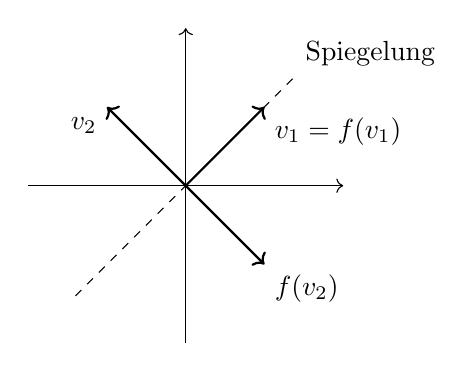
\begin{tikzpicture}
			\draw[->] (-2,0) -- (2,0);
			\draw[->] (0,-2) -- (0,2);
			\draw[dashed] (-1.4,-1.4) -- (1.4,1.4) node[anchor=south west] {Spiegelung};
			\draw[thick,->] (0,0) -- (1,1) node[anchor=north west] {$v_1=f(v_1)$};
			\draw[thick,->] (0,0) -- (-1,1) node[anchor=north east] {$v_2$};
			\draw[thick,->] (0,0) -- (1,-1) node[anchor=north west] {$f(v_2)$};
		\end{tikzpicture}
	Basis $(v_1, v_2)$ aus EVen mit EWen 1, -1, ${_\mathcal B}M_\mathcal B(f) = \twoXtwo{1}{ 0}
																						{0}{-1}$
	\item Drehung um Winkel $0 < \varphi < \pi$.\\
		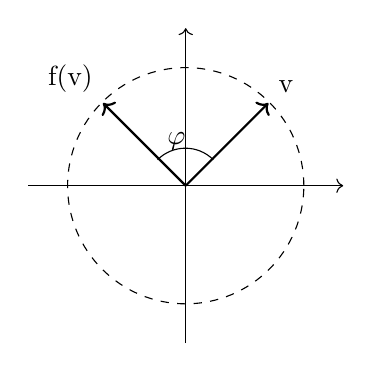
\begin{tikzpicture}
			\draw[->] (-2,0) -- (2,0);
			\draw[->] (0,-2) -- (0,2);
			\draw[dashed] (0,0) circle (1.5cm);
			\draw[thick,->] (0,0) -- (1.05,1.05) node[anchor=south west] {v};
			\draw[thick,->] (0,0) -- (-1.05,1.05) node[anchor=south east] {f(v)};
			\draw (0.35,0.33) arc (45:135:0.5cm) node[anchor=south west] {$\varphi$}; 
			%Es ist perfekt so wie es ist. Zahlen nicht hinterfragen!
		\end{tikzpicture}
	Keinerlei EVen
	\item Scherung \\
	$f(v) = \twoXtwo 	{1} {1}
						{0} {1} v$\\
		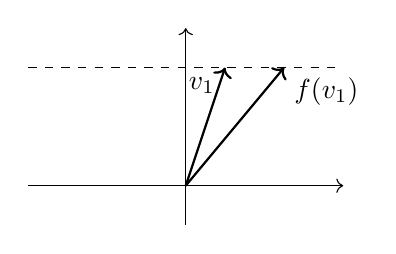
\begin{tikzpicture}
			\draw[->] (-2,0) -- (2,0);
			\draw[->] (0,-0.5) -- (0,2);
			\draw[thick,->] (0,0) -- (0.5,1.5) node[anchor=north east] {$v_1$};
			\draw[thick,->] (0,0) -- (1.25,1.5) node[anchor=north west] {$f(v_1)$};
			\draw[dashed] (-2, 1.5) -- (2, 1.5);

		\end{tikzpicture}		
	EVen nur $\vecTwo	{x}
						{0}$ (mit EW 1), die anderen "scheren aus".
				
\end{enumerate}
\subsection*{Bemerkung}
Ein Vektor $0 \neq v\in V$ ist EV von f zum EW $\lambda$ \\
$\Leftrightarrow v\in ker(f-\lambda\cdot id_V)$. mit $f-\lambda\cdot id_V:V\to V;\tn{ } v \mapsto f(v)-\lambda\cdot v$\\
Also $\lambda$ EW $\Leftrightarrow$ $f-\lambda\cdot id_V$ nicht injektiv.\\
Beweis klar, denn $(f-\lambda\cdot id_V)(v)=0 \Leftrightarrow f(v)-\lambda\cdot v=0$.
%----------------------------------Vorlesung 8----------------------------------
\end{document} 